% ----------------------------------------------------------
% ELEMENTOS PRÉ-TEXTUAIS
% ----------------------------------------------------------

% ---
% Capa
% ---
\imprimircapa
% ---

% ---
% Folha de rosto
% (o * indica que haverá a ficha bibliográfica)
% ---
\imprimirfolhaderosto%*
% ---
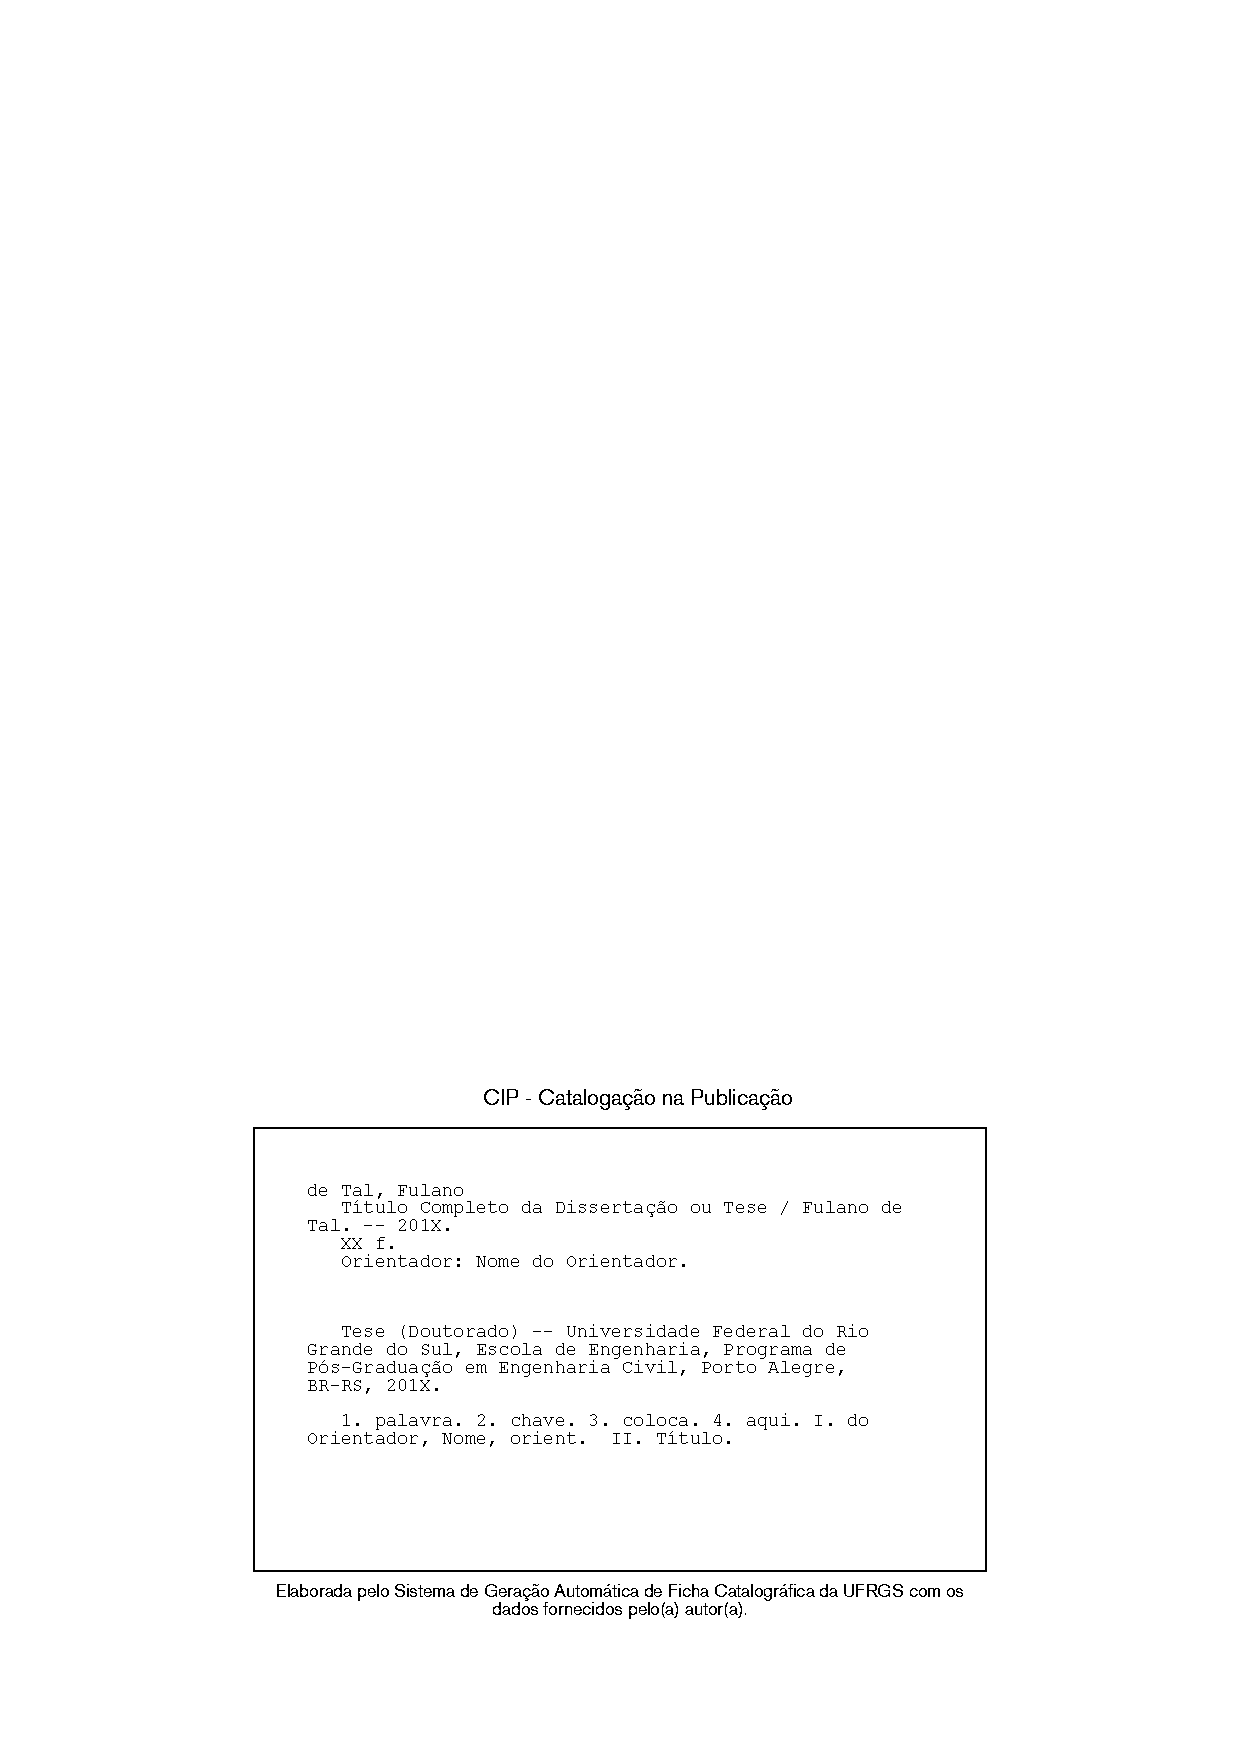
\includepdf[page={1}]{ficha}
% ---
% Inserir a ficha bibliografica
% ---

% Isto é um exemplo de Ficha Catalográfica, ou ``Dados internacionais de
% catalogação-na-publicação''. Você pode utilizar este modelo como referência.
% Porém, provavelmente a biblioteca da sua universidade lhe fornecerá um PDF
% com a ficha catalográfica definitiva após a defesa do trabalho. Quando estiver
% com o documento, salve-o como PDF no diretório do seu projeto e substitua todo
% o conteúdo de implementação deste arquivo pelo comando abaixo:
%

% --------------------
% \begin{fichacatalografica}
%     \includepdf{fig_ficha_catalografica.pdf}
% \end{fichacatalografica}

%\begin{fichacatalografica}
%	\ttfamily
%	\vspace*{\fill}					% Posição vertical
%	\begin{center}					% Minipage Centralizado
	% \fbox{\begin{minipage}[c][8cm]{13.5cm}		% Largura
	% \small
	% \imprimirautor
	%Sobrenome, Nome do autor

	% \hspace{0.5cm} \imprimirtitulo  / \imprimirautor. --
	% \imprimirlocal, \imprimirdata.

	% \thelastpage p.\\

% 	\hspace{0.5cm} \imprimirorientadorRotulo~\imprimirorientador\\
%
% 	\hspace{0.5cm}
% 	\parbox[t]{\textwidth}{\imprimirtipotrabalho~--~\imprimirinstituicao,
% 	\imprimirdata.}\\
%
% 	\hspace{0.5cm}
% 		1. Palavra-chave1.
% 		2. Palavra-chave2.
% 		2. Palavra-chave3.
% 		I. Sobrenome, Nome, orientador.
% 		II. Universidade xxx.
% 		III. Faculdade de xxx.
% 		IV. Título
% 	\end{minipage}}
% 	\end{center}
% \end{fichacatalografica}
% ---
% --------------------

% ---
% Inserir errata
% ---
% \begin{errata}
% Elemento opcional da \citeonline[4.2.1.2]{NBR14724:2011}. Exemplo:

% \vspace{\onelineskip}

% FERRIGNO, C. R. A. \textbf{Tratamento de neoplasias ósseas apendiculares com
% reimplantação de enxerto ósseo autólogo autoclavado associado ao plasma
% rico em plaquetas}: estudo crítico na cirurgia de preservação de membro em
% cães. 2011. 128 f. Tese (Livre-Docência) - Faculdade de Medicina Veterinária e
% Zootecnia, Universidade de São Paulo, São Paulo, 2011.

% \begin{table}[htb]
% \center
% \footnotesize
% \begin{tabular}{|p{1.4cm}|p{1cm}|p{3cm}|p{3cm}|}
%   \hline
%   \textbf{Folha} & \textbf{Linha}  & \textbf{Onde se lê}  & \textbf{Leia-se}  \\
    % \hline
    % 1 & 10 & auto-conclavo & autoconclavo\\
%   \hline
% \end{tabular}
% \end{table}

% \end{errata}
% ---

\begin{folhadeaprovacao}

  \begin{center}
    {\ABNTEXchapterfont\large\MakeUppercase{\imprimirautor}}

    \vspace*{\fill}
    \begin{center}
      \OnehalfSpacing{\ABNTEXchapterfont\bfseries\Large\MakeUppercase{\imprimirtitulo}}
    \end{center}
    \vspace*{\fill}
    \OnehalfSpacing{Esta \MakeTextLowercase{\imprimirtipotrabalho} foi julgada adequada para a obtenção do título de \MakeUppercase{\tituloobtido}, na área de concentração \areaconcentracao, e aprovada em sua forma final pelo professor orientador e pelo Programa de Pós-Graduação em Engenharia Civil da Universidade Federal do Rio Grande do Sul.}
    % melhorar o espaçamento entre linhas dessa parte
    \vspace*{36pt}
   \end{center}
    \begin{center}
    \imprimirlocal, \datacompleta
    \end{center}

    \begin{flushright}

    Prof. \imprimirorientador \\ \titorientador \\ Orientador
    \vspace{7mm}
    \\ Prof. \coordenador \\ \titcoordenador \\ Coordenador do \abrevppg/\abrevinstituicao
    \vspace{5mm}
    \\ \textbf{\MakeUppercase{Banca Examinadora}}
    \vspace{5mm}
    \\ \textbf{\tratbancaum~\bancaum~(\origembancaum)} \\ \titbancaum
    \vspace{5mm}
    \\ \textbf{\tratbancadois~\bancadois~(\origembancadois)} \\ \titbancadois
    \vspace{5mm}
    \\ \textbf{\tratbancatres~\bancatres~(\origembancatres)} \\ \titbancatres
    \vspace{5mm}
    \\ \textbf{\tratbancaquatro~\bancaquatro~(\origembancaquatro)} \\ \titbancaquatro

    \end{flushright}

    \vspace*{\fill}
    \vspace*{\fill}


  \end{folhadeaprovacao}
%   ---